\documentclass{acm_proc_article-sp}
\usepackage{algorithmic}
\usepackage{algorithm}
\usepackage{listings}
\usepackage{booktabs}
\usepackage{graphicx}
\begin{document}

\title{On Reallocation of Resources during Releases \titlenote{Permission to make digital or hard copies of all or part of this work for
personal or classrooms use is granted without fee provided that copies are not made or distributed for profit or commercial advantage and that copies bear this notice and the full citation on the first page. To copy, to republish, to post on servers or to redistribute to lists,
requires prior specific permission and/or a fee. Copyright \copyright 2013}}
\numberofauthors{2}
\author{
% 1st. author
\alignauthor
Md Tajmilur Rahman\\
       \affaddr{Concordia University}\\
       \affaddr{Montreal, QC H3G 1M8}\\
       \email{mdt\_rahm@encs.concordia.ca}
% 2nd. author
\alignauthor
Peter C. Rigby\\
       \affaddr{Concordia University}\\
       \affaddr{Montreal, QC H3G 1M8}\\
       \email{peter.rigby@concordia.ca}
}
\date{20 Oct 2013}
\maketitle
\begin{abstract}
Software projects often suffer from lesions in software industries due to disruptive events what may occur naturally or because of managerial directions. Keeping this in mind we have taken an approach to examine the development process of a large software project to understand the nature and behavior of the process and distribution of resources within the different areas of the system. By using the historical data from the distributed version control (DVC) system used by that large project we quantify aspects of developers' distribution, code ownership, different release periods, focus on the areas of the code-base, percentage of working with owned files during different periods withing a release cycle for this project. This study reveals a unique process performing well extraction of data from Git for the development of a large open source project by which we can perceive significant points of information that can lead us to further decisional analysis aiming novel solutions to the disruptive events for the practitioners of software development.

\end{abstract}
\category{K.6.3}{Software Management}{Software Development, Software Resource Management, Resource Reallocation}
\terms{Experiment, Human Factors, Resource Management, Reallocation}
\keywords{Resource Reallocation, Code Ownership, Software Releases} % NOT required for Proceedings
\section{Introduction}
Software projects are notorious for going over budget and schedule. Rush periods are often get seen before a major release that turn the developers into dinosaurs as Frederick Brooks likens in his benchmark study ``The Mythical Man Month'' \cite{brooks_mythical}. This ``Rush To Release (RTR)'' can be prompted either by external forces such as decisions by management to include new features in the release or to release earlier to beat a competitor. Alternatively, the rush may simply be due to inappropriate or unrealistic scheduling. Whatever the reason is it is an obvious. Regardless of the causes, the rush to release stresses developers and often requires developers to work on unusual, high priority or critical areas of the system. In this paper we study how RTR may effect project organization to introduce technical debt. We want to propose a method to observe, analyze and summarize the results found around different parts of a release cycle. We intend to infer behavior of the developers related to the process around release time. The key research questions that we expect to answer with our methodology are described in section 1.1.

During the development period, developers are free to make any change that might go for release. Around the time of release, we generally would expect fixes on the code files those have been worked on during the development. In this study we observe the developers' working areas to understand their allocation and contribution within an open source software development project to understand the development process, nature of reallocation of resources or (i.e.\ developers), change in work strategy during different period of a release cycle especially during the time of release, developers' focus on the code-base in a large software project which may cause disruptive events. The historical data that we have worked on for this purpose will help us to extract a lot of information that will help us to understand the role of the developers, code ownerships of the domains they are working in, density of work, nature of dealing with files dealing around the time of release etc.

We have organized this paper as follows. In section 2, we describe some background and motivations followed by the summaries of related works in section 3. Section 4 will describe methodology of our work and explanation of the data we are working with for this research. In section 5 we will discuss the results of the findings. We are describing our limitations and threats to validity in section 6 and finally section 7 will conclude the paper.

\subsection{Research Questions}
We have set our research questions focusing the key properties of software development process, allocation of developers throughout the development and release, especially for open source software development. First couple of research questions are to understand the basic structure and strategies of the development and release and merging process practiced by Linux Kernel developers. Rest of the questions are to understand the distribution of developers', working areas and the behavior of developers during different segments of a release cycle.

\renewcommand{\labelenumi}{RQ\theenumi:}
\begin{enumerate}
\item What is the release process used by the project? \newline
We will be giving a qualitative description of Linux Kernel development in brief to answer this question.
\item How many developers are allocated throughout different segments of a release cycle? What significant difference can be observed between the segments of a release cycle? \newline
Answer to this question will give us a brief information of Linux Kernel development community as well as the contribution of developers in different parts within a stable release.
\item Do developers work on different areas of the system around the time of release? \newline
We want to see if developers are looking at different types of files in the code-base around the time of release which is being considered as the release period. We are going to introduce an algorithm to traverse through the git DAG to find out commits associated to a particular release. This can be useful for any other data collected from distributed version control system like git.
\item Do developers work in others' code in a high proportion during the rush period?\newline
Developers work on various files during release period. We will try to find out what is the percentage of dealing with files that developers own or they are most familiar to. This will give us a sense of the nature of work during the release time.
\item How long a commit takes to get pushed into the master branch? Does it differ in different periods of release?\newline
In distributed development environment developers work in different branches. They commit their codes to the branches they are associated to. While core development is going on developers do not directly push their changes to the main branch. We would like to see how much time it takes for a commit to the local branch to get pushed to the main branch. We also compare between how long it takes for regular development commits and how long it takes for the commits made during the release period.
\item Are there certain areas of the system that receive increased attention (i.e.\ do developers focus on a smaller set of files around releases)? \newline
To answer this question we will look into the files getting churned extremely high in number. We will try to figure out the difference between those highly churned or highly focused sets of files in different releases to understand if they require constantly high focus or they are for a particular release only.
\end{enumerate}

\section{Background}
There may have lower developers productivity \cite{cataldo_identification, damian_awareness} which may cause inefficient run in the rush moments in a release period. There is a substantial and important body of literature on risk in software engineering. Boehm identified the most important risks encountered by software project managers and described successful risk management practices \cite{boehm_software_risk, keil_framework, boehm_agile}. Some of the risks identified are related to disruptive events, such as the introduction of a new technology, but most are macro risks associated with running a project, such as developing the wrong functionality. General risk mitigation strategies can be difficult to apply to specific disruptive events. There may be various kinds of disruptive events for example, as a release approaches; developers take shortcuts that introduces technical debt. If it is not repaired, the long term quality of the system will suffer. Another example can be placed, if a lead developer who owns an important part of the code-base leaves and if steps to train other developers were not taken, it will become a dead area of the system and will be difficult to modify and maintain. Also often management reorganizes the developers on a company's projects during the rush period around the release time, as a result that developers move to code areas for which they have less experience. The reorganization introduces new perspectives and expertise that can lead to faster release; however, it can also result in a drop in productivity and the unnecessary re-writing of large portions of the system that the new developers do not understand. In our study, we plan to take the measures on this last example among all mentioned above.

\section{Related Works}
Hindle worked on release pattern discovery via partitioning \cite{hindle_release_pattern} to propose an approach to characterize a project's behavior around the time of major and minor releases while we are trying to study the behavior of the development resources around the time of release. In this research they proposed a method of observing, analyzing and summarizing the results of metrics of revisions found near releases. They have characterized a project's behavior around the time of major and minor releases. This is done by partitioning the observed activities like the artifact check-ins around the dates of major and minor releases, then look for reasonable patterns. Hindle divided the revisions in each release in 4 different classes, Source Code, Testing, Building, and Documentations. On the other hand Cook did an interesting job, he inserted sensors and monitors into the development process but Hindle analyzed the data to understand what happened in the past \cite{cook_automating}. Basically Hindle worked in a reversed way than Cook did.

Another research work we would like to mention was done by  Damian where they have worked on the role of domain knowledge and cross functional communication among the OOS development teams \cite{damian_domain}. Posnett did some dual ecological measures of focus in software development \cite{posnett_ecological}. Posnett's measure was for the more general view that unifies developers' focus and artifact ownership. He analyzed i) developer artifact contribution to network to a predator-prey food web ii) drew upon ideas from echology to produce a novel and iii) conceptually unified view of measuring focus and ownership. Another study was done by F. Rahman about the authorship of the code-base in OSS development \cite{rahman_ownership}. This is one of the main focuses of our method for this study. We have used code ownership to understand the hold of the developers on the system. Not only code ownership but we also focused on the percentage of working with owned files during the release time and what is the percentage of working with owned files when developers provide increased attention to the code files around the time of release.

\section{Methodology}
This section presents our methodology for discovering information which can give us the idea to get the answers to our research questions. We have collected the development historical data of Linux Kernel. It is a data source containing the the historical data of Linux kernel development since 2005. We are going to present the steps involved in this process and then we will follow up with an application of our methodology as a case study. In order to address our research questions, we obtain key measures of project evolution from the archival data collected from the distributed version control (DVC) system of Git where all information of the OSS project ``Linux Kernel Development'' is recorded in electronic form. Many other OSS projects archive similar data, so the techniques being used by us can be replicated on other projects as well. We used the data elements extracted from the archival source to construct a number of measures on the commit log records to understand the distribution and behavior of the developers.

Our methodology can be summarized as: Extracting Data for revisions and releases (Section 4.1); Partitioning the release version numbers (Section 4.2); Finding the commits associated to a version of Kernel (Section 4.3); Get time-span between each release (Section 4.4); Calculate developer areas (Section 4.5); Finding code ownership (Section 4.6).

\subsection{Data Extraction}
We collected the data downloading every revision and commit log history data. From DVCSs such as Git we extract the revisions and release information. We wrote Perl scripts to extract date and managed them in Postgre SQL database to create tables in, to store our extracted data. These extracted data will be analyzed by us later on. For each revision the information extracted includes the commit id, tree id, author of the revision, date of revision, the name of the revised file, parent and child info for the revision and the detail log information. Once extraction is completed we are ready to partition the version numbers (Section 4.3) and duration  of each release (Section 4.4).

\subsubsection{Explanation}
A Linux kernel development release version constructed with maximum length of information does look like \textbf{linuxvA.B.C-rcP} where A, B, C, P are numeric. If a release version looks like ``linuxv2.6.13'' it tells us that this particular release is the 13th micro release in the series of the 6th minor release of kernel version 2. ``linuxv2.6.13\textbf{-rc1}'' says that after the 12th stable minor release published, development for the next release has been ended all new files are merged and rc1 is the first candidate release that starts working on the next release, basically it starts the release period. We have last couple of release candidates for ``linuxv2.6.12'' and first couple of release candidates for ``linuxv3.12'' which is not useful for our calculation. So we are having 340 releases including major, minor, micro and rc. 39 stable releases from ``linuxv2.6.11'' to ``linuxv3.11'' having complete data with us. We have total 400441 distinct commits and for 372943 of them have change information for 77082 different files in our hand where we have 13926 developers' commit history among 14621 distinct developers. Surprisingly 14569 individual files didn't have any change (addition or deletion) but was being committed at least once. So we found them in our released wise datasets.

 \subsection{Partitioning Release Numbers}
We stored the extracted git commit log data into the tables git\_commit and git\_revision where all the basic and detail log information for a particular commit was mentioned in the first table and second one containing which commit belongs to which version of Linux kernel development and change details like path modified, new path created due to the change, how many addition and how many deletion occurred in a particular commit etc. By joining these two tables we can easily get the dates of each release version and from the version number we can determine which commit belongs to which version and release, and also what type of release that is.

Commits those are made for pushing a release have release tags associated to them by which makes us understand which commit is made for a release and also if it is a major or minor or a micro stable release. Another information we have captured that is \textbf{rc} which indicates that the particular commit was a release candidate. These information and splitting off the release numbers will help us accumulating commits associated to different releases.

\subsection{Finding Commits for Releases}
We have sorted out and accumulated all the commits together belonging to any of the releases. We have all 400441 commits in our hand but though we can't plot them into a single time domain to assign different set of commits to different release periods because development goes in parallel on different branches in git, so commits also go in parallel.
\begin{figure}
\begin{center}
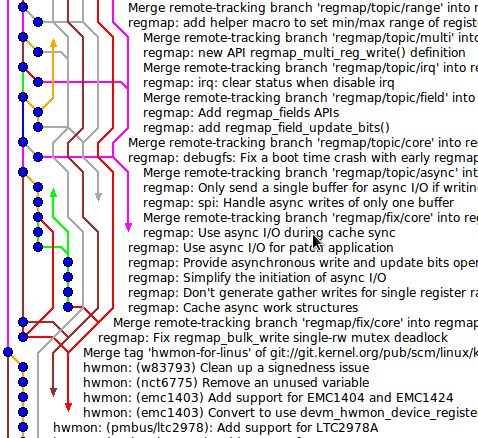
\includegraphics[height=2.5in,width=2.5in]{gitdag.png}
\caption{\small \sl Branching in git DAG for linux kernel development.}
\end{center}
\end{figure}
If there are multiple branches, surely there are multiple merges and the commits prior to a crisscross merge are all ancestors of the heads of all subsequent branches \cite{bird_git}. Figure 1 shows how a git DAG looks like having so many crisscross merges in a busy branching snap-shot of the git DAG of Linux Kernel development.

It is possible to make a commit months ago while several releases may have already been made in the mean time but that commit can belong to any future release. Commits that are being made to a development branch may get merged with the head branch during the merge period. This is why we had to track all the way down the trees for each of the 340 releases in the git DAG to find out which commit contributes to which release. We could do this using Git DAG Traversing (GDT) algorithm as described in Algorithm 1. After applying GDT we collected 381152 commits out of 400441 those are well organized in the git DAG of Linux Kernel development. As we mentioned earlier that we have last couple of release candidates for ``linuxv2.6.12'' and first couple of release candidates for ``linuxv3.12'' those we are chopping out because we don't have complete commit records for the release cycle linuxv2.6.12 releases as well as linuxv3.12. Out of 400441 commits 19289 are belonging to those releases. Therefore, finally we have 381152 commits for 331 releases in our database to progress our work on where 39 release are stable.
\begin{algorithm}
\caption{GDT: Git Dag Traversing}
\begin{algorithmic}[1]
\REQUIRE
\STATE commit id for all releases
\ENSURE
\FOR{all commits}
\STATE start from new commit, release R
\STATE store commit in ``git\_commit\_release''
\IF{has parent commit}
	\FOR{each parent commit}
		\IF{if parent commit has a release tag}
			\STATE repeat step 1
		\ELSIF{parent commit already stored}
			\STATE compare release versions
			\IF{release version not smaller than R}
				\STATE update existing\_release $\gets$ R
			\ENDIF
		\ELSE
			\STATE store parent commit in ``git\_commit\_release''
			\STATE commit id $\gets$ parent commit id
			\STATE repeat step 3
		\ENDIF
	\ENDFOR
\ELSIF{no parent commit}
	\STATE repeat step 1
\ENDIF
\ENDFOR
\end{algorithmic}
\end{algorithm}
\subsection{Time-Span of Releases}
Another information that we require is what are the durations of the releases of Linux kernel development. To achieve that we joined the table ``git\_refs\_tags'' where all the releases are stored including the release numbers and the table ``git\_commit'' to give us all the dates of commits for each and every releases, so that we can easily find out the duration between two consecutive releases (including release candidates ``rc''). This information will significantly help us because we need to see what is the development period and what are the release periods within a release cycle. We also need to understand how developers are working, what is the impact of their changes made in the code-base during a particular release period later on. Table 1 shows a small portion of this information. Prior to calculate the developers' areas in section 4.4 we need this information.

\begin{table}[ht]
\caption{Different Releases}  	% title of Table
\centering 						% used for centering table
\begin{tabular}{c c c c}				% centered columns (4 columns)
\hline\hline						%inserts double horizontal lines
% table heading
Release & Type & Start Date & End Date \\ [0.5ex]
\hline 							% single horizontal line
% inserting body of the table
linuxv2.6.12-rc2 	& rc       	& - & 2005-04-16 \\
linuxv2.6.12-rc3 	& rc       	& 2005-04-16 	& 2005-04-20 \\
linuxv2.6.12-rc4 	& rc       	& 2005-04-20 	& 2005-05-07 \\
linuxv2.6.12-rc5 	& rc       	& 2005-05-07 	& 2005-05-24 \\
linuxv2.6.12-rc6 	& rc       	& 2005-05-24 	& 2005-06-06 \\
linuxv2.6.12     	& micro 		& 2005-06-06 	& 2005-06-17 \\
linuxv2.6.13-rc1 	& rc       	& 2005-06-17 	& 2005-06-29 \\
linuxv2.6.13-rc2 	& rc       	& 2005-06-29 	& 2005-07-05 \\
linuxv2.6.13-rc3 	& rc       	& 2005-07-05 	& 2005-07-13 \\
...			     	& ...	   	& ... 		    & ...\\
...			     	& ...	   	& ... 		    & ... \\
...			     	& ...	   	& ... 		    & ... \\
linuxv3.11          	& minor 	& 2013-08-25 		& 2013-09-02 \\
[1ex]							% adds vertical space
\hline 							% inserts single line
\end{tabular}
\label{table:nonlin} 			% is used to refer this table in the text
\end{table}

Note that the very first row has no information for the ``Start Date'' because we don't have the  complete information prior to stable release ``linuxv2.6.12'' and we have chopped them out. This will not affect our methodology and measurements. From the extraction we found complete records for releases ``linuxv2.6.13'' to ``linuxv2.6.39'' then it is ``linuxv3.0'' to ``linuxv3.11''. Our farther works will be proceeded based on these 39 stable releases.

\subsection{Developers' Area}
Developers are working throughout the all the time. Some are working during the release period, at the same time some people may be working for any new feature development for any future release. Here ``Developers' Area'' means the files developers work in those are going to be merged in a release. It doesn't refer to the file itself but it is important to understand which files are being touched by which developers. We see that authors are committing files almost everyday throughout a release but this does not make sure that these commits are going to the next release because commits are being made in different branches and all branches are not supposed to get merged to the next release. Using GDT algorithm we have acqumulated all the commits finally went to a particular release. Now it is possible to find out which commits were made for which files by which developer for a release.

A relatively straightforward discipline of Linux Kernel Development team is followed with regard to the merging of patches for each release \cite{linux_kernel}. At the beginning of each development cycle, the "merge window" is said to be opened. At that time, code which is deemed to be sufficiently stable (and which is accepted by the development community) is merged into the mainline kernel. The bulk of changes for a new development cycle (and all of the major changes) will be merged during this time, at a rate approaching 1,000 changes ("patches," or "change-sets") per day. Strategically Linux starts a new kernel release with the merging to get their development branch ready to start development for the next release. So there are two main segments in a release period, one is merge window or development period (DP) where all the developments works get merged together from different branches. So we can say this is the main development period of a release. A development period remains opened exactly for two weeks \cite{linux_kernel}, many developers are working in many other branches to develop new features once they are ready to push it to the main kernel then they wait for the upcoming merge window and once it's development period they all contribute their works for the next release during this Development Period. Some developers who are mainly responsible to merge new developments verify and accept the new changes and merge them into the main kernel. Another perod in a release cycle is the period of candidate releases which gets opened once the merge window is closed where mainly the bug fixing of minor enhancement works are to be worked on and pushes by small candidate releases. Once all the fixing and enhancements are done for all the codes that had been merged into the main kernel, the release is published. We are calling this part of a release cycle as the release period (RP) because no new feature development works get accepted during this time, it is just the period prior to publishing a new release.

\subsubsection{Developers' Area in a Development Period}
Development Period can be determined from the previous release date (of any of major, minor or micro releases) to the date of rc1 (i.e.\ date of the first candidate release). For example if the date of release for ``linuxv2.6.12'' is 2005-06-17 and date of pushing the rc1 for the next release ``linuxv2.6.13'' is 2005-06-29 then this time period of of 12 days is going to be called as the merge window or development period. Thousands of commits get pushed in the main branch during this period. Table 2 shows the development periods of some releases.

\begin{table}[ht]
\caption{Development Periods (Merge Window)}  % title of Table
\centering 						% used for centering table
\begin{tabular}{c c c c}				% centered columns (4 columns)
\hline\hline						%inserts double horizontal lines
% table heading
Release 			& Start Date		& End Date \\ [0.5ex]
\hline 							% single horizontal line
% inserting body of the table
linuxv2.6.13		& 2005-06-17	& 2005-06-29 \\
linuxv2.6.14		& 2005-08-28	& 2005-09-12 \\
linuxv2.6.15		& 2005-10-27	& 2005-11-11 \\
linuxv2.6.16		& 2006-01-02	& 2006-01-17 \\
linuxv2.6.17		& 2006-03-20	& 2006-04-02 \\
linuxv2.6.18		& 2006-06-17	& 2006-07-06 \\
linuxv2.6.19		& 2006-09-19	& 2006-10-04 \\
linuxv2.6.20  		& 2006-11-29	& 2006-12-13 \\
linuxv2.6.21		& 2007-02-04	& 2007-02-20 \\
linuxv2.6.22		& 2007-04-25	& 2007-05-12 \\
linuxv2.6.23		& 2007-07-08	& 2007-07-22 \\
linuxv2.6.24		& 2007-10-09	& 2007-10-23 \\
linuxv2.6.25		& 2008-01-24	& 2008-02-10 \\
[1ex]							% adds vertical space
\hline 							% inserts single line
\end{tabular}
\label{table:nonlin} 			% is used to refer this table in the text
\end{table}

We have the commits contributed to releases and every record explains us who committed the file when did this get churned. If we run an SQL query then we can easily find out for every author and for every particular file how many times a it has been committed by an author and how many churns (lines added + lines deleted) a developer has made. We calculate developers' working areas and store the information into a table. A part of that table is shown in table 3.

\begin{table}[ht]
\caption{Developers' Areas in Development Period}  % title of Table
\centering 						% used for centering table
\begin{tabular}{c c c c}				% centered columns (4 columns)
\hline\hline						%inserts double horizontal lines
% table heading
Author		& File Path			& Commits		& Churn \\ [0.5ex]
\hline 							% single horizontal line
% inserting body of the table
D. S. Miller	& include/.../pci.h		& 1				& 8 \\
V. Hanquez	& arch/.../cpu.c		& 1				& 14 \\
A. Bunk		& drivers/.../shmem.c	& 1				& 2 \\
J. Juhl		& arch/.../generic.c		& 1				& 3 \\
[1ex]							% adds vertical space
\hline 							% inserts single line
\end{tabular}
\label{table:nonlin} 				% is used to refer this table in the text
\end{table}

In this table we see, in a development period within a release cycle D. S. Miller has made change in ``pci.h'' file only once where he has made 8 churns. In the similar approach we calculate developers' areas in release period.

\subsubsection{Developers' Areas in Release Period}
As like development period we can extract developers working in code files during release period. Release Period here in Linux Kernel development process is being considered as since the date of rc1 release (i.e.\ first release candidate opening the gate for the development of the next release) to the date of the next stable release. For example if the date of rc1 for ``linuxv2.6.13'' after releasing ``linuxv2.6.12'' is 2005-06-29 and the date of publishing the release ``linuxv2.6.13'' is 2005-08-28 then we are calling this 60 days of development period for the release as the Release Period. Table 4 is showing some development periods of different releases.

\begin{table}[ht]
\caption{Release Periods}  % title of Table
\centering 						% used for centering table
\begin{tabular}{c c c c}				% centered columns (4 columns)
\hline\hline						%inserts double horizontal lines
% table heading
Release 			& Start Date		& End Date \\ [0.5ex]
\hline 							% single horizontal line
% inserting body of the table
linuxv2.6.13		& 2005-06-29	& 2005-08-28 \\
linuxv2.6.14		& 2005-09-12	& 2005-10-27 \\
linuxv2.6.15		& 2005-11-11	& 2006-01-02 \\
linuxv2.6.16		& 2006-01-17	& 2006-03-20 \\
linuxv2.6.17		& 2006-04-02	& 2006-06-17 \\
linuxv2.6.18		& 2006-07-06	& 2006-09-19 \\
linuxv2.6.19		& 2006-10-04	& 2006-11-29 \\
linuxv2.6.20  		& 2006-12-13	& 2007-02-04 \\
linuxv2.6.21		& 2007-02-20	& 2007-04-25 \\
linuxv2.6.22		& 2007-05-12	& 2007-07-08 \\
linuxv2.6.23		& 2007-07-22	& 2007-10-09 \\
linuxv2.6.24		& 2007-10-23	& 2008-01-24 \\
linuxv2.6.25		& 2008-02-10	& 2008-04-16 \\
[1ex]							% adds vertical space
\hline 							% inserts single line
\end{tabular}
\label{table:nonlin} 				% is used to refer this table in the text
\end{table}

These information above will greatly help us to answer our first couple of research questions and to progress our further works.

\subsection{Finding Code Ownership}
So many developers are working from different development communities throughout different development branches. We tried to investigate the ``code ownership'' \cite{mockus_case_study} evolved in Linux Kernel development. Here code ownership is going to be represented as a percentage of making churns by a developer with respect to the total churns made to a particular file. From the data of all 39 releases we found 70210 distinct files have been churned by developers. We removed those files where no developer made any churn at all during these 39 releases. We investigate the total number of churns for each and every file, we also investigate how many developers contributed for these commits and changes. This information yet does not tell about the ownership, we need to find out ownership for each developer in different development areas in a release cycle. We already have the collection of developers working in development period and release period within a release cycle and stored them with corresponding files they have worked on, how many commits a developer made to a particular file and how many changes he/she has made. We now update those information with the ownership information. Equation 1 is the base for calculating ownership.
\begin{equation}\omega=\frac{n}{N}*100\end{equation}
Where $\omega$ is the ownership and n is the number of total changes made by an atuthor of a file, N is the total number of changes made for a particular file.
To determine a developer be a owner of a file we are considering that if the developer makes changes more than 80\% of the total churn that has been made by all contributors so far for that file, then that developer can be called as a owner of that file, similarly as C. Gutwin did \cite{gutwin_awareness} for finding out the main developers' group for a project. We calculate code ownership for both Development Period and Release Period. We also calculate general ownership for all the developers for all the files they have worked ever. Table 6 represents a part of the data which shows the ownerships of the developers in each release cycle.

\begin{table}[ht]
\caption{Code Ownership in Release Period}  % title of Table
\centering 						% used for centering table
\begin{tabular}{c c c c}				% centered columns (4 columns)
\hline\hline						%inserts double horizontal lines
% table heading
Author 				& Linuxv		& Path				& $\omega$ (\%) \\ [0.5ex]
\hline 							% single horizontal line
% inserting body of the table
Thomas Gleixner		& 2.6.24		& .../numa\_64.h		& 0.0000\\
Jeff Kirsher			& 3.1		& .../ethtool.c		& 0.0000\\
Sathya Perla			& 2.6.29		& .../hwlib.h		& 100.00\\
Roel Kluin			& 2.6.24		& .../innovator.h 	& 100.00\\
David S. Miller		& 2.6.24		& .../visasm.h 		& 100.00\\
Stephen Hemminger	& 2.6.24		& .../qla3xxx.c	 	& 12.083\\
Randy Dunlap			& 2.6.24		& ...\_core.c 		& 100.00\\
[1ex]							% adds vertical space
\hline 							% inserts single line
\end{tabular}
\label{table:nonlin} 			% is used to refer this table in the text
\end{table}
The example given above is calculated for finding ownerships of developers worked for different files in different releases. Ownership is calculated for all the developers in release periods as well as in development period. In addition we have calculated which file is owned by which developer and also the percentage of working with owned files during development and release period separately. These extractions will help us drawing the results from our findings to answer our 3rd and 4th research questions.

\section{Results}
In this section we present results from several quantitative analysis of the archival data from the Linux Kernel development project. The measures we derive from these data are well-suited to answer our research questions.

\textit{What is the release process used by the project?}

In the early 1990's the Linux kernel development was not so busy affair \cite{linux_kernel}. There were very small number of users and developers involved at that time. Developers use a loosely time-based release process. Linux publishes it's major kernel release in every two or three months. If we look at figure 2 the upper Line represents how the stable releases are going on since 2005. From the figure we can see the average duration of each stable release is 62.47 although ``linuxv2.6.24'' was significantly hight as exception, it took 92.8 days. The bottom line which is much steady than the upper one is representing the durations of development period in each stable release. If we put the releases in a time domain we can see a picture shown in figure 2 where we see that the stable releases are all going on maintaining almost a similar frequency and similar pattern. The highest picks are the development periods then the smaller picks between the highest ones are representing the rc releases. For more clear view we have plotted only 100 releases of 331 releases including release candidates.

\begin{figure}
\begin{center}
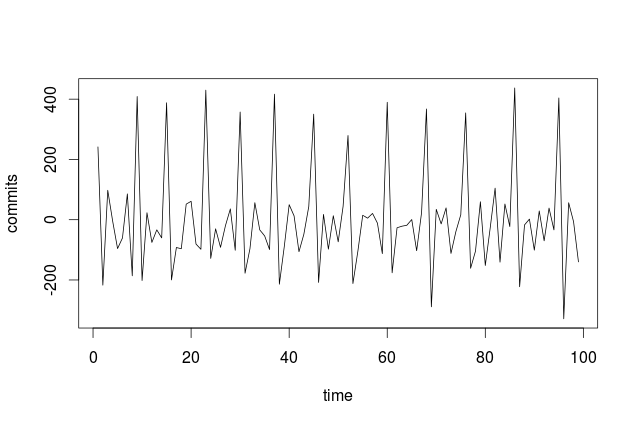
\includegraphics[height=1.7in,width=3.4in]{relTimeDomain100.png}
\caption{\small \sl Time Domain for Releases}
\end{center}
\end{figure}

Linux Kernel development uses ``Rolling Release Development Model''. Usually every micro release (ex.\ linuxv2.6.x) is a major kernel release with new features, internal API changes, and more. A minor release (ex.\ linuxv3.11) can have around 10 thousand change-sets with several hundred thousands of churned lines of codes (LOC). At the beginning of each stable release the merge window i.e.\ development period gets opened and all the accepted and stable codes from the community are merged having around 1000 of churns everyday. Development period approximately for 14 days as shown in the figure 3. The bottom line is representing the merge windows of every releases. We don't have the development period data for the very first one that's why it's starting from 0.

\begin{figure}
\begin{center}
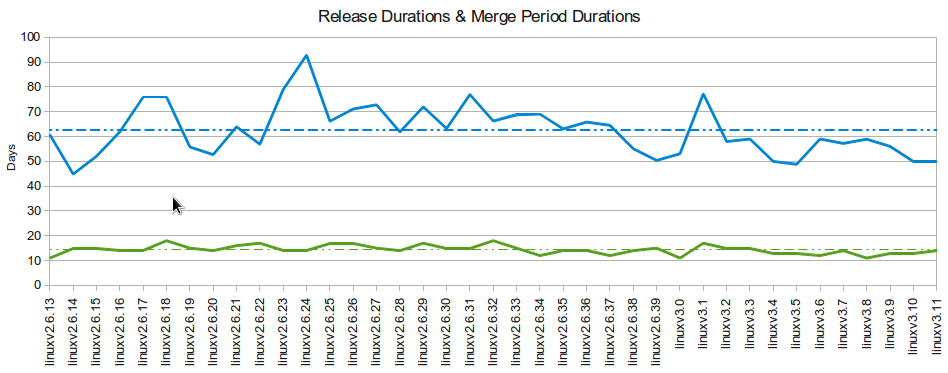
\includegraphics[height=1.7in,width=3.4in]{linxrelmergfreq.png}
\caption{\small \sl Durations of Merge Window and Release Cycle}
\end{center}
\end{figure}

After getting all the major works merged, release period for the next release is announced to be opened. If the next release is going to be linuxv2.6.14 then the release pushed out at the end of the merge window will be called linuxv2.6.14-rc1. \textbf{rc1} indicates that all the new features or developments are merged now the time to stabilize the next kernel has begun. These candidate releases continue to be pushed for once a week. If there is any bug fix or any high-priority change only then that goes to the main line during this period. With the continuous rc releases when the new kernel seems to be stable then it goes to publish the next stable release. Again merge window gets opened and accepts more new features, patch-sets from different branches.

As a summary, the description above helps us to address some of the questions about how Linux Kernel development is organized. Answer to this first research question provides essential background for understanding our quantitative results. We will look into more detail of the development process, distribution of developers among the release segments as well as will try to find answers for our other research questions in the next sections.

\subsection{Difference Between Release Segments}
\textit{How many developers are allocated troughout different segments of a release period? What significant difference can be observed between the segments of an entire release cycle, also between two consecutive releases?}

In order to see how many developers contribute to the new feature developments and how many contribute in merging and fixing, review and accepting codes from the community during the development period, we observed the developers' area in Development Period and developers' area in Release Period. Out of all 381152 commits belonging to 331 releases 292926 commits were made during the time of development period which is 76.85\% (more than 2/3) of the total. These commits were made by 13926 individual developers, 11209 developers work in development periods and 7625 developers work around the release periods.

In figure 4 we see the boxplot showing that a very large number of developers contribute during the development period which is in a sense the main development period because all the development branches get merged together during this time, all the new features come into the main branch of the kernel. In release period significantly small number of developers work and this number looks pretty steady for all the releases only a couple of high number appeared in two releases as we see in figure 4. The number of contributions during the main development period over releases looks going up in an increasing manner as shown in figure 5. On the other hand the bottom line for the release developers is pretty steady for all the releases.

\begin{figure}
\begin{center}
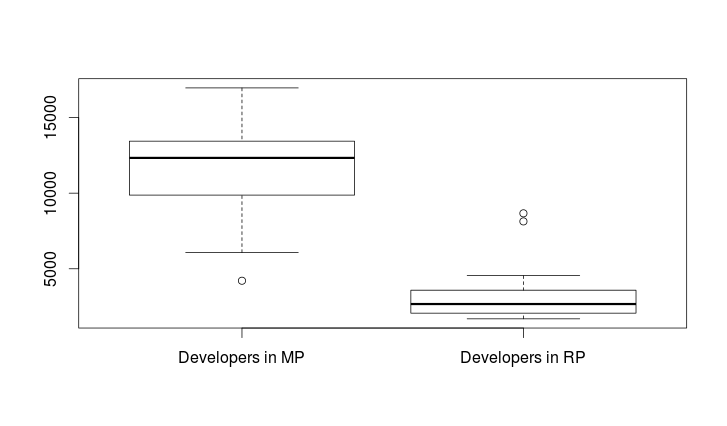
\includegraphics[height=1.7in,width=3.4in]{devsMPRPbox.png}
\caption{\small \sl Developers working in DP \& RP}
\end{center}
\end{figure}

\begin{figure}
\begin{center}
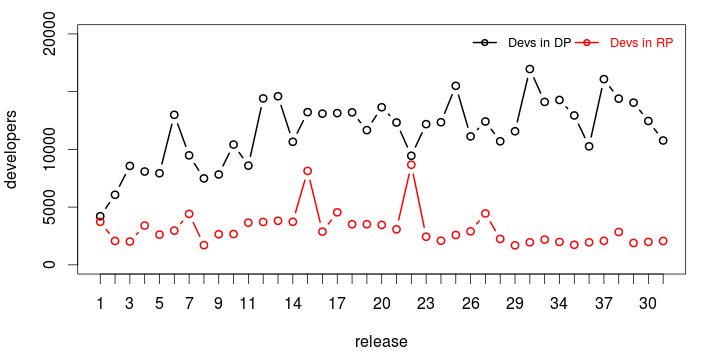
\includegraphics[height=1.7in,width=3.4in]{devsMPRP.png}
\caption{\small \sl Increasing contribution in DP}
\end{center}
\end{figure}

Once we found different releases and the release periods as well as we calculate the developers' areas and code ownerships for developers we also would like to know what is the difference being created by making changes between the two main segments within an entire release cycle. To observe this we want to calculate the difference using Jaccard Similarity Coefficient \cite{jaccard_alpine} which is represented by equation 3.
\begin{equation} J(A, B) =\frac{|A \cap B|}{|A \cup B|} \end{equation}
The Jaccard Distance can be obtained by subtracting the Jaccard Coefficient from 1.
\begin{equation} d_j(A, B) = 1 - J(A, B) = \frac{|A \cup B|-|A \cap B|}{|A \cup B|} \end{equation}
Here A and B are two sets. For calculating Jaccard distance between two releases we are considering the files that have been worked for, in a particular release. If set A is the set of files worked in DP and files worked for in another release is set B then In figure 6 the Jaccard distances between Development Period and Release Period for each release can be represented. The average jaccard distance between development period and release period for all the release cycles is 0.85 and we see the Jaccard distance is also going upward by releases except the only exception at release 2.6.34.

\begin{figure}
\begin{center}
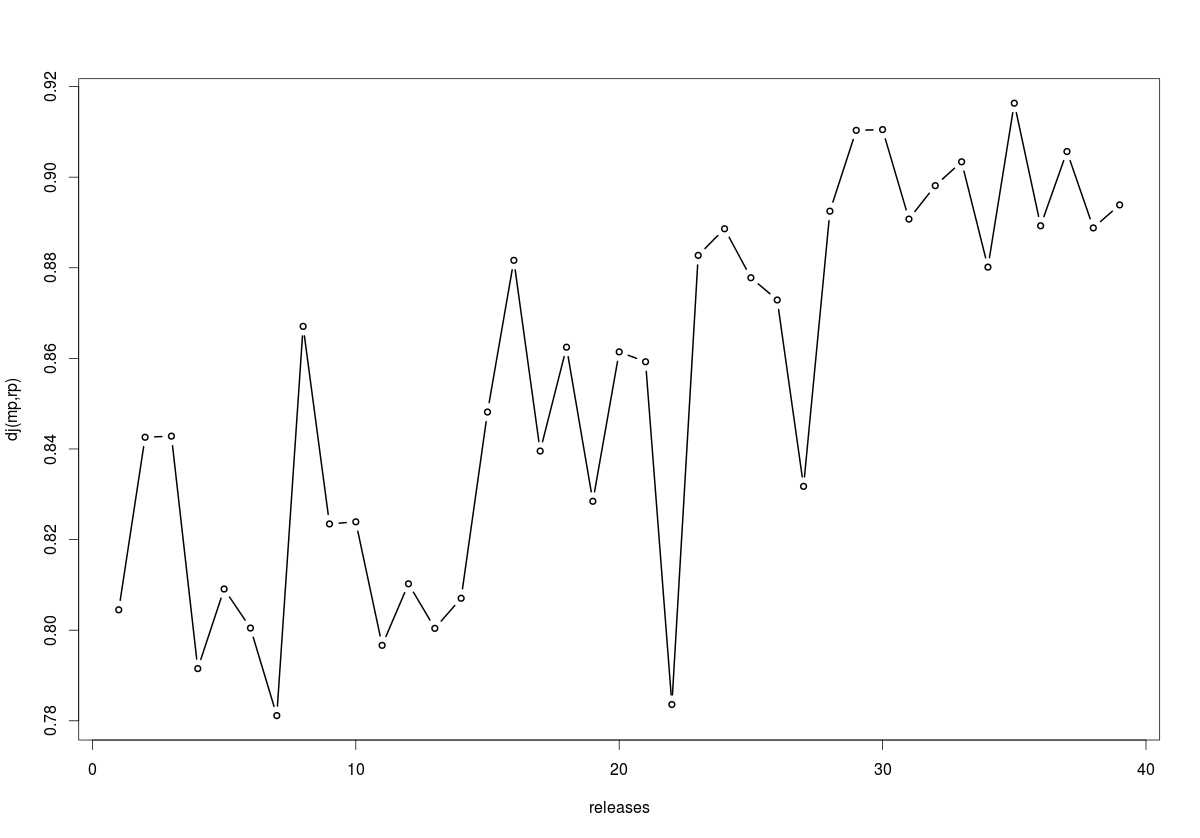
\includegraphics[height=1.7in,width=3.4in]{jdMPRP.png}
\caption{\small \sl Jaccard Distance between the Development Period and Release Period}
\end{center}
\end{figure}

\subsection{Developers' Contributions Around the Time of Release}
\textit{Do developers work on different areas of the system around the time of release?}\newline
\textit{Do developers work in others' code in a high proportion during the rush period?}

We are supposed to find the answers for the two research questions together in this section. Developers work for the software continuously. Some are working for the core development some people are for the fixing and minor enhancements and some for feature developments, planning to merge new features with any up coming release but we would like to understand what number of files they change during the time of development and merging period and how many during the release period. How many of them they really own and how many files they work that they do not own. We also want to know about the code ownership of the developers around the time of release as well as around the time of main development works that get merged during development period.

In order to understand the distribution of the developers around the system we also found that during these release periods 11209 developers have experience of working in the development period and 7625 developers worked in the release period as we already mentioned earlier but we noted that 4908 developers contribute in both development period and the release period that means near about half (43.78\%) of the developers work during the development period are shared that means they work for core developments and also bug fixing or minor enhancement works. Figure 7 representing the venn diagram.
\begin{figure}
\begin{center}
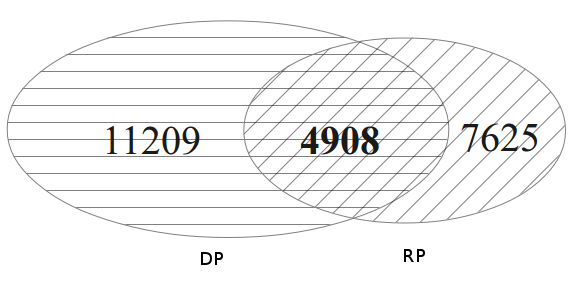
\includegraphics[height=1.3in,width=2.3in]{devDistMPRPvenn.png}
\caption{\small \sl Developers' Distribution in Development Period and Release Period}
\end{center}
\end{figure}

From release ``linuxv2.6.13'' to ``linuxv3.11'' We examine the contribution in writing code by the developers to understand the behavior during the two vital segments in a release cycle. Figure 8 plots the cumulative representation of the percentage of working with owned files ($\omega$\textit{MP}) during the development period and the percentage of working with owned files ($\omega$\textit{RP}) during release period of ``linuxv2.6.13''. From the figure it can be observed that with the increase of every 10 files that developers working in, $\omega$\textit{RP} is going down apart from the line of $\omega$\textit{MP}. Up to a certain number may be around 2200 files developers mostly work with owned files. We see the similar picture for other releases too.
\begin{figure}
\begin{center}
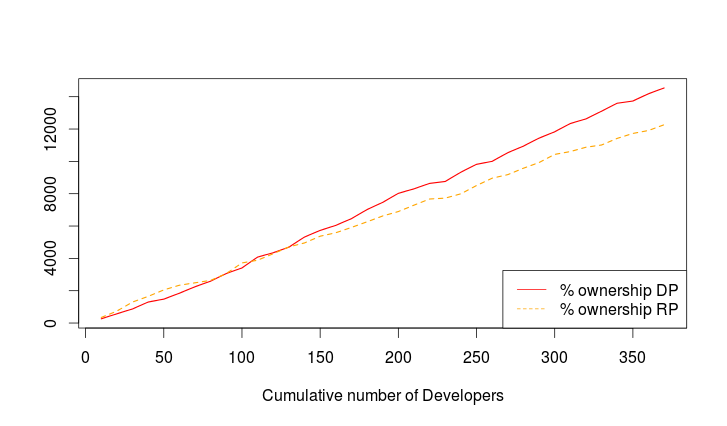
\includegraphics[height=1.7in,width=3.4in]{cumulFileOwnP.png}
\caption{\small \sl Cumulative percentage of working with owned files in DP and RP of release 2.3.13}
\end{center}
\end{figure}

If we simply compare the percentage of working in owned files during development period ($\omega$\textit{MP}) and the percentage of working in owned files during release period ($\omega$\textit{RP}) for each developer then we see a significant difference of the mean lines as shown in figure 10. In release period developers work with less number of files that they own.

To obseve the similarity of files being worked on in different development periods of releases we can have a look at figure 9. Here x axis represents the consecutive release pairs and y axis for the Jaccard similarity index. In this figure we see the line which is representing the jaccard similarity index for files being worked in consecutive development periods is upper enough to the line representing jaccard similarity index for files being worked in consecutive release periods. Which does make sense that around the time of release developers work in more in different and random files that's why possibility of the similarity with the files that are worked in previous release's RP and the files that are worked in current release is very low.
\begin{figure}
\begin{center}
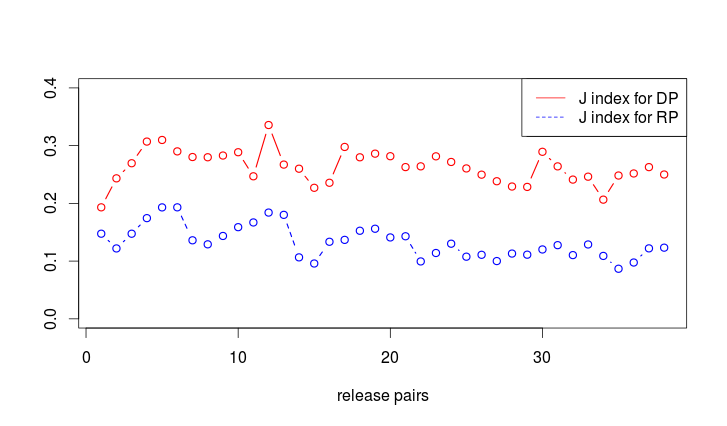
\includegraphics[height=1.7in,width=3.4in]{j_file_MPMPvRPRP.png}
\caption{\small \sl Jaccard similarity index between consecutive releases (for both DP and RP). X-axis: consecutive release pairs, Y-axis: J-index}
\end{center}
\end{figure}
So we can say that in Linux Kernel development developers work in more unfamiliar files during the release period. Before the release period starts main development works are accepted from different branches and they get merged together with the main kernel thus core feature developers finish their duty for a particular feature development for a particular release within the time of development period although some contributors still work during the release period where basically they work on fixing, testing and minor enhancement related work on the codes that have been merged and accepted from various developers from other branches. It is clear now that during the release period developers work mostly on others' works, the proportion of working with owned files is lower around the release than the proportion during normal development time. When they feel the confidence that everything is tested and can be pushed out for the release, they publish the stable release.

\begin{figure}
\begin{center}
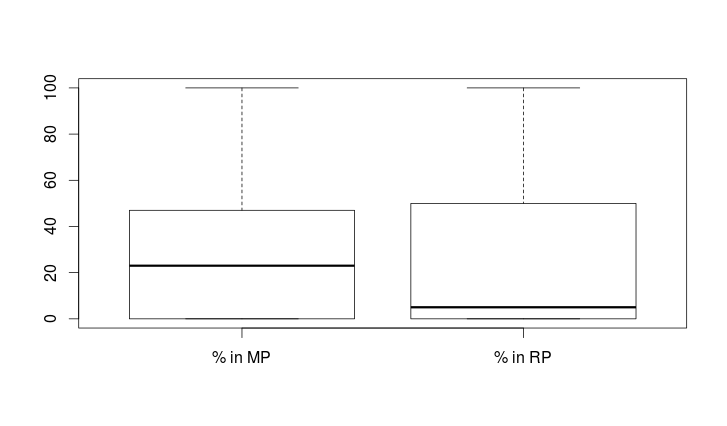
\includegraphics[height=1.7in,width=3in]{ownpMPRPbox.png}
\caption{\small \sl Percentage of working in owned files during Development Period and Release Period}
\end{center}
\end{figure}

So, finally we can say that in development periods developers work in more native codes while during the release development period the percentage of working with native code is very low in number although this percentage of working in owned code during development period does not significantly relate to other co-factors.

\subsection{Time for Commits to Go Live}
\textit{How long a commit takes to get pushed into the main kernel? Does it differ in different periods of release?}

There are thousands of commits goes to the main kernel during the merge window. All they are to be considered as the normal development commits or regular development or core development commits for developing new features to the kernel. Merge window remains opened for two weeks only, the development works that are supposed to go for a particular release are not developed during this couple of weeks. These have been developed since many days ago on a different development branch by any developer. For a particular feature that is going to the current release there are hundreds of commits, obviously all these commits are not made during the merge window of the current release 90-100\% commits must have been made before the opening of the merge window of current release. As described in section 4.3, we have sorted up the releases according to the git DAG. This helps us to calculate how many days in past the first commit of this particular feature had been made which is going to be pushed into the current release. The duration a commit was made to the local branch to the date it is pushed into the main branch is being called here ``lag'' of commits. Figure 11 represents lag of the commits made for regular development and lag of the commits made during the release period.

\begin{figure}
\begin{center}
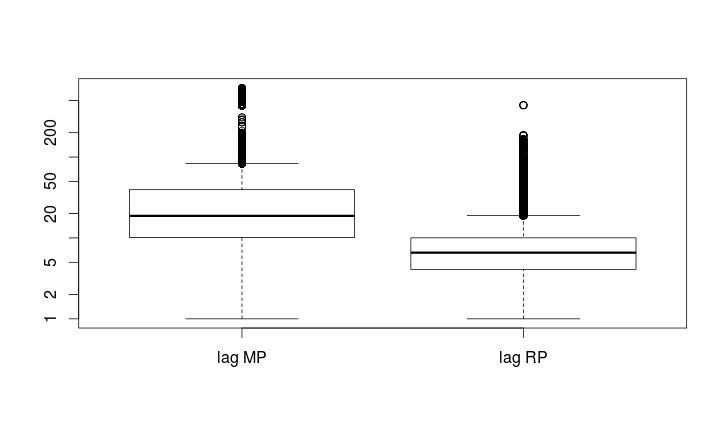
\includegraphics[height=1.7in,width=3in]{lagMPRPbox.png}
\caption{\small \sl Time takes for development commits and commits around release periods to get released}
\end{center}
\end{figure}

From figure 10 we can understand that quick fixes are made during the release period. With the small sets of bug fixes, important quick enhancements candidate releases are pushed continuously within short lengths of time and once the kernel seems to be more stable with all the new features that has been merged during the beginning of the release cycle, the stable release is published. Comperatively lag for the feature development commits is quite high. Median for the lags for the commits during this time is 5.57 while median of the lags for the commits going to the main kernel of the development  period is 26.15, which is a significant difference between these two parts of a release cycle.

\subsection{Developers' Focus on Code-Base Around the Time of Release}
\textit{Are there certain areas of the system that receive increased attention (i.e.\ do developers focus on a smaller set of files around releases)?}

To answer this research question we are interested to find answer to the following questions first.
\renewcommand{\labelenumi}{q\theenumi:}
\begin{enumerate}
\item{How many churns were made to the files during release periods?}
\item{How many files get churns exceptionally high in number? Do we see this in every release cycles?}
\item{How many files each developer deals with during release development period?}
\item{How many files developer deal with large number of files during release development period? What is the percentage of ownership of them while working for a large number of files in a release period?}
\item{If there is any area that requires increased attention in the system, then what is the Jaccard distance of those areas throughout different releases? Are they being focused iteratively by releases?}
\end{enumerate}

During the time of rc releases after all the merging jobs are done developers generally work for minor fixing and serious quick enhancements. In all these 39 release cycles of Linux Kernel development wee see in an average 3077 churns are made around the releases. The minimum value is 1691 and maximum is 8669. Median and mean values are closer enough (2668 and 3077) to say that almost similar kind of churns are made in all the release periods except couple of exceptions. If we look at figure 12 where the normalized distribution of this data is represented then we can easily understand this.
\begin{figure}
\begin{center}
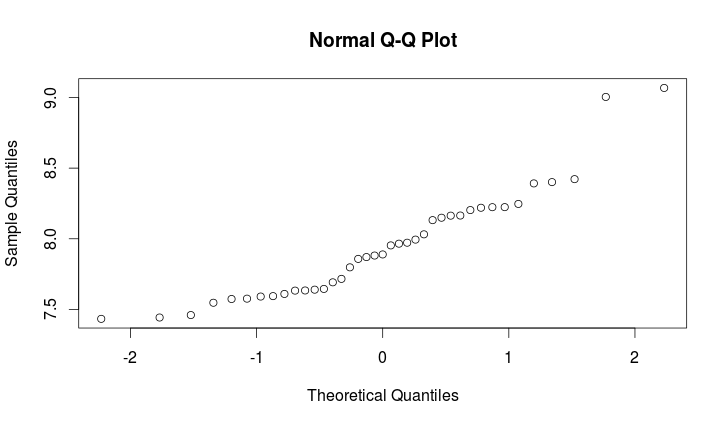
\includegraphics[height=1.7in,width=3in]{churnRPnorm.png}
\caption{\small \sl Normal distribution of churns per Release Period}
\end{center}
\end{figure}

We analyzed several release cycles and found that during the release period of ``linuxv2.6.13'' 2938 files got churned. Among them only five files had exceptionally high number of churns four of them have more than 10,000 churns. Usually around 2000 files are worked on during the release periods except 2 releases where the number of churned files was extremely high. For almost every release cycle during the release period around 2.846 files get highly increased attention having over 5000 churns and 16.78 files having over 1000 churns as shown in figure 13. Similar picture we see for other releases also. But, if some one renames a file containing thousands of lines of codes and then just commits it then we will see the churn is as many lines as the file contains. In Linux Kernel development, the code files related to device drivers are just copied or renamed because these files are mainly reused or just the license informations added. In this case they usually get committed once or twice. As we see in tha data throught all the releases there are 621 instances where a file has got more than a thousand churns and 466 of them have less than 5 commits and most of those files are for different kinds of device configuration or drivers related files. So, to calculate highly focused files we are considering number of commits instead of churns. We think at least this will make sense that how many times developers are getting involved to a file around the time of release which describes the focus more than churns.

For each stable releases, number of files having more than 10 commits during the release period can be plotted as we see in figure 14. In an average 12.92 files get more than 10 commits around every release period although during few release periods we have seen around 35 even 50 files got commits more than 10 times.

\begin{figure}
\begin{center}
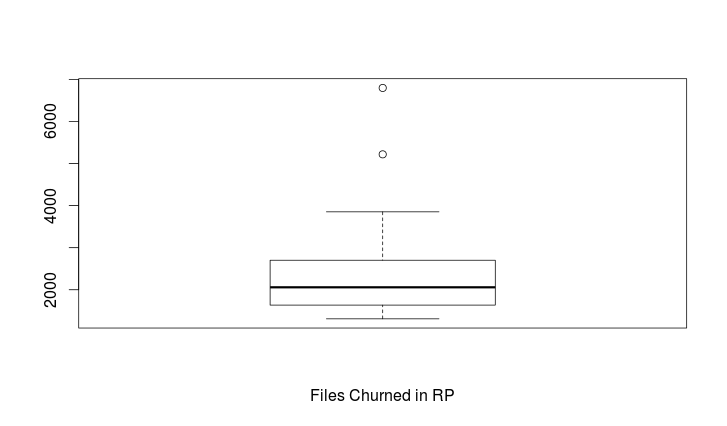
\includegraphics[height=1.7in,width=3in]{fileChurnRPbox.png}
\caption{\small \sl Number of Files churned in release periods}
\end{center}
\end{figure}

\begin{figure}
\begin{center}
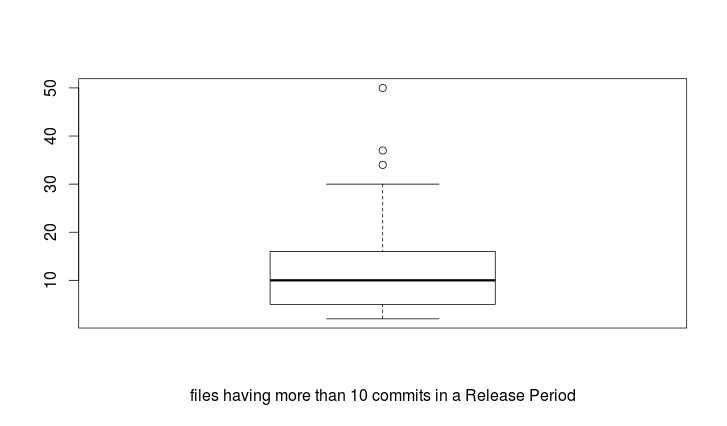
\includegraphics[height=1.7in,width=3in]{file_commit_exeptional_rp10box.png}
\caption{\small \sl Files committed more than 10 times during release period}
\end{center}
\end{figure}

During the release period developers deal with various files came from different authors working in different development branches in merge window. Although the number of files developers deal with during release period is too low (mean 5.52) there is a large number of developers work for around 50 files. To look for how many developers work for fairly large number of files we decided to see which developers work for more than 100 files in the release periods.

We found that there are 29 releases out of the 39 where developers are working in comparatively large number of files during the release period? Among them we noted that 5 developers in 5 different release periods worked for extremely high number of files as listed in table 6. In this table we also have represented what is the percentage of working with owned files for each developer.

\begin{table}[ht]
\caption{Developers making churn in extremely high number of files during Release Periods}  % title of Table
\centering 						% used for centering table
\begin{tabular}{c c c c}				% centered columns (4 columns)
\hline\hline						%inserts double horizontal lines
% table heading
Author 						& Linuxv		& Owned 			& Total \\
							& 			& Files				& Churned \\ [1ex]
\hline 							% single horizontal line
% inserting body of the table
Greg Kroah-Hartman			& 3.8		& 70\%				& 1114\\
David Howells				& 2.6.19		& 38\%				& 1140\\
Russell King					& 2.6.27		& 70\%				& 2426\\
Lucas De Marchi				& 2.6.39		& 64\% 				& 2466\\
Tejun Heo					& 2.6.34		& 34\% 				& 4222\\
[1ex]							% adds vertical space
\hline 							% inserts single line
\end{tabular}
\label{table:nonlin} 				% is used to refer this table in the text
\end{table}

So, we can say that there are certain areas of the system that takes certainly increased attention also there are few developers who deal with large number of files at the time of release. Some of them work less than 40\% files that they own and some developers work around 70\% of files that they own. Now we would like to see if these areas having increased attention get the similar attention in other releases. This finding also supports our fourth research question \textit{RQ4} strongly. In this occasion we would like to find the Jaccard similarity index for these highly focused areas in between two consecutive releases. First we collected the sets of files those are having highly increasing churns during the release periods of different release cycles and also the sets of files that are getting high number of commits. Then we calculated the union and intersection operation between two sets for two consecutive releases. We applied equation 2 to find out the similarity among the sets. For the sets we collected based on churns, we don't see any similarity between them except for couple of pairs of releases where the Jaccard indexes are 0.038, 0.066, 0.025 and 0.181 respectively as shown in figure 15.

\begin{figure}
\begin{center}
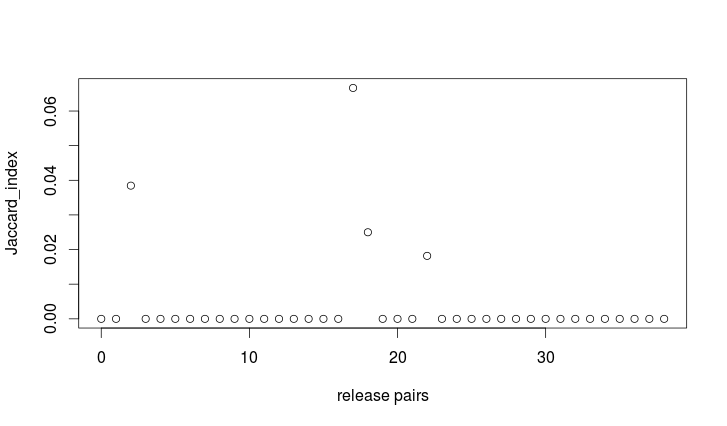
\includegraphics[height=1.7in,width=3.4in]{jdRPChurnHighFocusFiles.png}
\caption{\small \sl Jaccard similarity index between consecutive sets of files having highly increased focus (based on churns) in different releases}
\end{center}
\end{figure}

But for the sets of code files we collected based on commits, we see positive Jaccard indexes for all consecutive release pairs which means some of the files those are receiving increased focus during the release period also receives highly increased focus in the later releases too. Figure 16 is representing this behavior.

\begin{figure}
\begin{center}
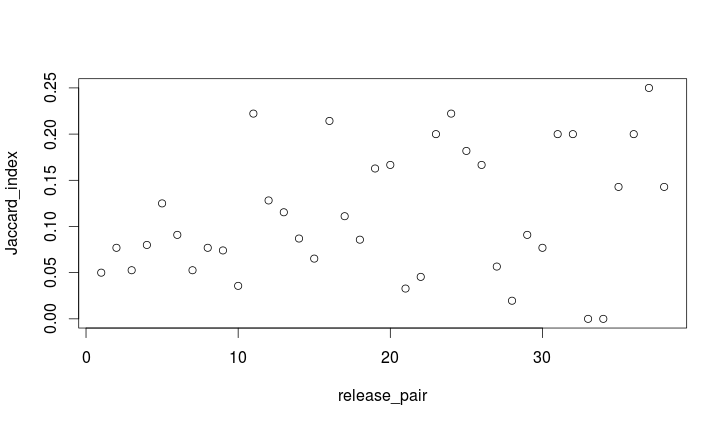
\includegraphics[height=1.7in,width=3.4in]{jdRPCommitHighFocusFiles.png}
\caption{\small \sl Jaccard similarity index between consecutive sets of files receiving highly increased focus (based on commits) in different releases}
\end{center}
\end{figure}

After all these results we can say that developers working for different and various features, developing new staffs for Linux kernel working in many different files and merging them into the main kernel during merge window. In release period small number of developers who are allowed to work in release period are reviewing those newly merged codes and doing quick fixes and enhancements. Some of them may require very high attention and more work to do. In the next release more different and new developments arrive in merge window and thus in release period developer keep pushing their candidate releases focusing on those newly arrived code files where there may have some files require more focus may be they received high focus in the previous release too.

\section{Threats to Validity}
Throught the paper we have done number of measurements to analyze the structure of an OSS software project development, behavior of the developers in different parts of the system, allocation and re-allocation of resources around the time of release as well as around the time of development. Now, are these measurements and findings really meaningful? Are they quantifying what we want them to?\newline\newline
\textbf{Construct Validity} To study the distribution and allocation of developers or resources around the development system for a large project, the very initial step should be understanding the project development strategy which project data we are studying on. Looking for the answer to our first research question is an obvious in this context where we clearly understood the history and flow of the development process of Linux Kernel, what are the durations of every release how can we distinguish different parts within a release cycle and so on. Once we get the different segments or distinguishable parts of a release cycle we feel the urgency to understand their external and internal behaviors also the relation of the resources, role of developers around them. Our second research question tells us every details on these and our third, fourth and fifth research questions take us more into the deep of this analysis to discover some core points of information from where we may start thinking of something different that may help us to progress our work farther more by setting any goal based on new hypothesis to come up with any decision. Our last research question is really giving us some meaningful discoveries to plot the critical true scenario of developers with code-base of a software project.\newline\newline
\textbf{Internal Validity} Is there any cause and effect relation between the changes in certain attributes and the results that we represented? In our methodology we actually picked few attributes like version of the release, sable release and candidate release, release commits, different periods within a release cycle like merge window or development period and release period, ownership, lag for commits in different periods, percentage of working with owned files during development and release periods, file churns, highly increasingly focused files, Jaccard distance between the sets of files of these types. The first attribute ``versions'' may vary with many other software projects so the data extraction model that we have used may not me similar to other projects but the GDT algorithm that we have used for acqumulating the commits associated to releases will be useful for other software projects having Git as the version control system.\newline\newline
\textbf{External Validity} We wanted to understand the allocation and re-allocations of the resources around the release of a software project we wanted to make a study with a large project and so we started our study with Linux Kernel development where we got approximately 400441 commit records made by thousands of developers for 340 releases (including stable and candidates). Can we generalize our results to other software projects? Although we looked into a large open source software, this is only one system we looked into. We need to analyze the development strategy and distribution of resources for others software projects also. We have plan to go for similar kind of analysis on other historical projects both OSS and non-OSS to generalize our findings and results by cross-validation across projects. We believe that the process we used for finding commits associated to a release tag (GDT Algorithm) will be re-usable for other projects using DVC.\newline\newline
\textbf{Reliability} The data we used for our study is highly reliable. It has been derived from the version control system that Linux Kernel development using. Other projects using similar version control system can easily run the same experiments to produce findings specific to those projects and to compare with our findings.\newline\newline
\textbf{Limitations} The results and findings of our study is currently based on a single project due to the limited access to such rich historical data. We hope to study more other OSS projects as well as non-OSS projects to ensure the validity and generality of our findings in the future.

\section{Conclusions}
Software development in a large team is really a complex process to deal with. Resource re-allocation is an important phenomenon in regard of software development especially in a large development environment. The results have been reported with respect to our research questions in this case study. We want to mention as a summary the following items have been reported by our measurements:
\renewcommand{\labelenumi}{\theenumi.}
\begin{enumerate}
\item{The basic structure and the development process of Linux Kernel.}
\item{The distribution of developers in two different segments in a complete release cycle.}
\item{Role of developers during development period and the significance of release period.}
\item{Developers' focus around the time of release, percentage of working with native code during development period and release period.}
\end{enumerate}
We intended to find out some points of crucial information that may lead us to move forward to come up with any new hypothesis or any decision about the rush period of release and the distribution of developers having in-equal hold on the code-base of the system which is strongly related to the disruptive events occur in software development industries. We have discovered a lot of information with good potentials to progress our research furhter more. We also were concerned about the developers' highly increased focus in code areas of the system that may create technical debts and we could see in our results that files having highly focus around the release periods are being handled by developers who may have high percentage of familiarity with them or may not also some of these files accepts increasing attention in the later releases too. Calculating the developers' focus on code area during the release period has been more meaningful as we are doing it based on commits instead of high number of churns because during this period high number of churns are made mostly due to the cloning of existing device/drivers configuration codes or due to very minor changes like signature or license statement change. We would like to investigate these matters in future to come up with more significant discoveries possibly with new decisional ideas about the disruptive events of software systems.

\bibliographystyle{abbrv}
\bibliography{paper1} 

\balancecolumns
\end{document}